% !Mode:: "TeX:UTF-8"
\documentclass{xcumcmart}
\usepackage{setspace}
\usepackage{enumerate}
\usepackage{graphics}
\usepackage{tabu}

% \title{text}这里是显示在第三页的文章标题
\title{相机成像原理}
\author{何长鸿 2016141482154}

\linespread{1.2} %行距
\CTEXsetup[format={\Large\bfseries}]{section} %章节标题左对齐
\setlength{\parskip}{1.4em} %1.4倍段落距离

\begin{document}
\renewcommand\arraystretch{2}
\maketitle

\section{改变焦距对拍照的影响}
\par 参数$cx=cy=50$固定不变,分别改变fx、fy并拍照得到如图\ref{fig:2255}到\ref{fig:1255},可以看到减小fx,图像在x方向上变窄,减小fy,图像在y方向变窄,同时减小fx和fy则整个图像减小。此处图像越小,则对应照片分辨率越低。因此,改变焦距会改变拍摄图像的分辨率。
\begin{figure}[htbp]
\centering
\begin{minipage}[htbp]{0.48\linewidth}
    \centering
	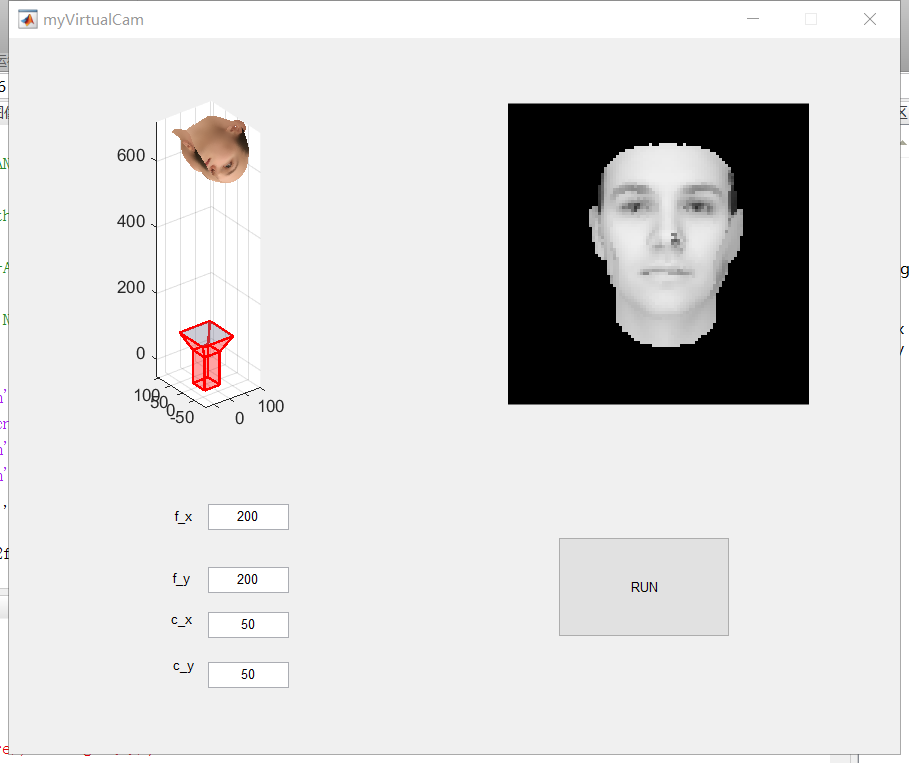
\includegraphics[width=1\textwidth]{fig/2255.png}
	\caption{fx=fy=200\label{fig:2255}}
\end{minipage}
\hfill
\begin{minipage}[htbp]{0.48\linewidth}
    \centering
	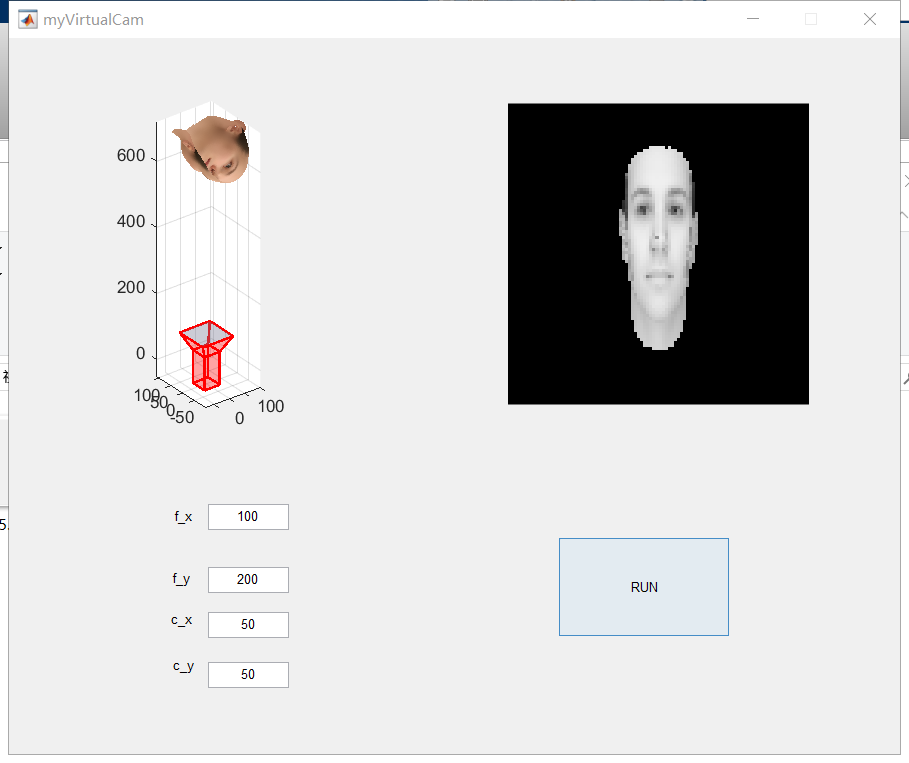
\includegraphics[width=1\textwidth]{fig/1255.png}
	\caption{fx=100,fy=200\label{fig:1255}}
\end{minipage}
\end{figure}
\begin{figure}
\begin{minipage}[htbp]{0.48\linewidth}
    \centering
	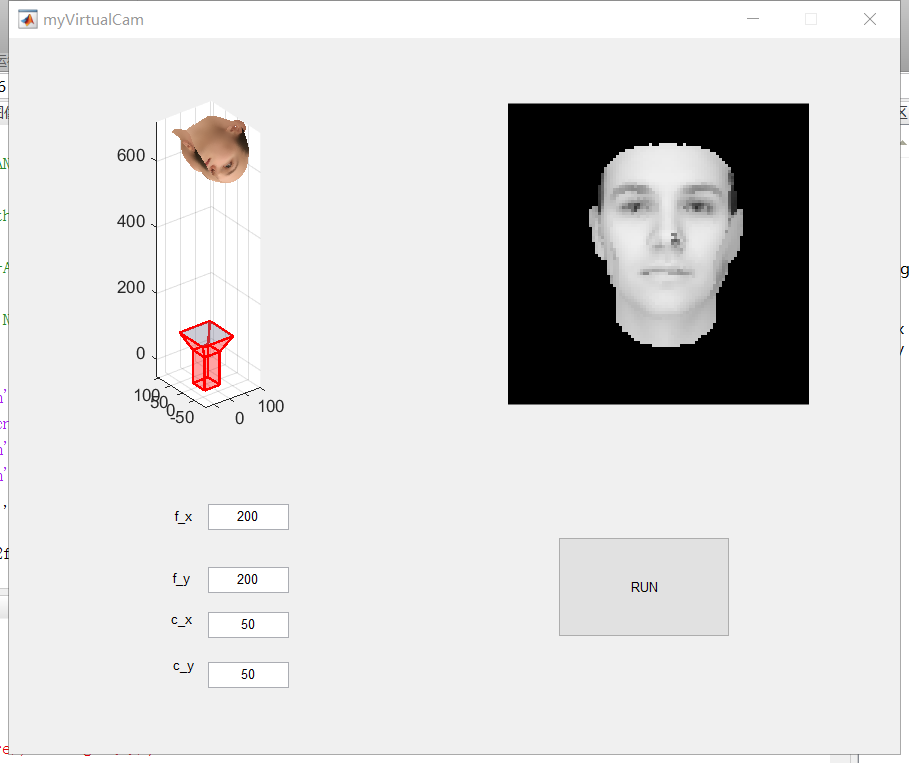
\includegraphics[width=1\textwidth]{fig/2255.png}
	\caption{fx=fy=100\label{fig:1155}}
\end{minipage}
\hfill
\begin{minipage}[htbp]{0.48\linewidth}
    \centering
	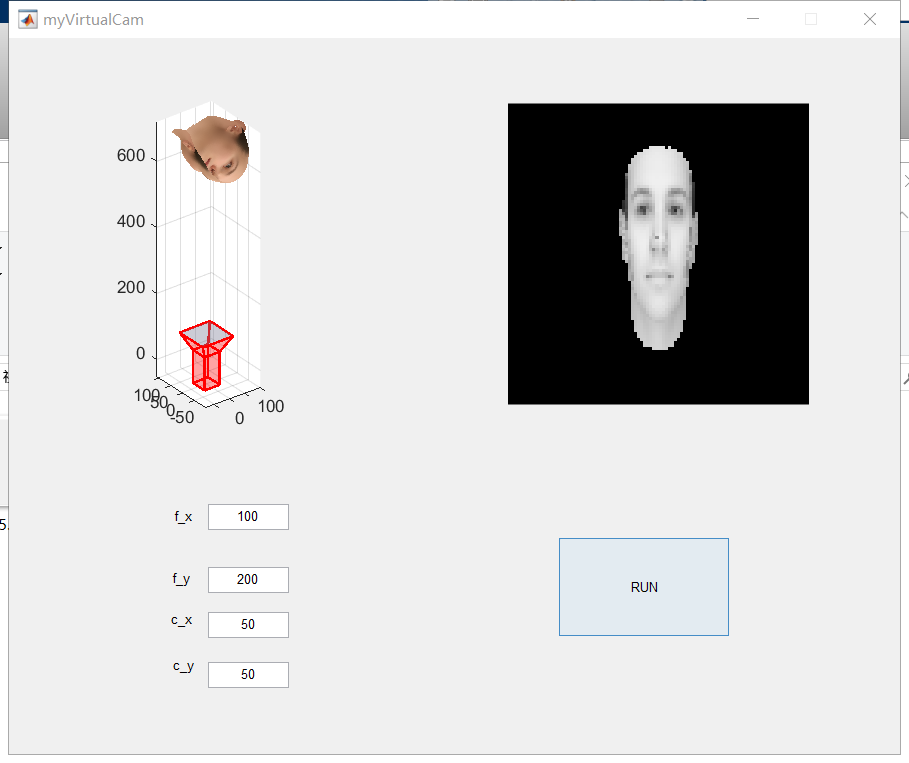
\includegraphics[width=1\textwidth]{fig/1255.png}
	\caption{fx=200,fy=100\label{fig:2155}}
\end{minipage}
\end{figure}


\section{改变主点对拍照的影响}
\par 参数$fx=fy=100$固定不变,分别改变cx、cy并拍照得到如图\ref{fig:1155-}到\ref{fig:1111},可以看到减小cx,图像向左下角运动,减小fy,图像向右上角运动,同时改变fx和fy则整个图像没有变化。因此,改变主点位置会改变拍摄图像的成像位置
\begin{figure}[htbp]
\centering
\begin{minipage}[htbp]{0.48\linewidth}
    \centering
	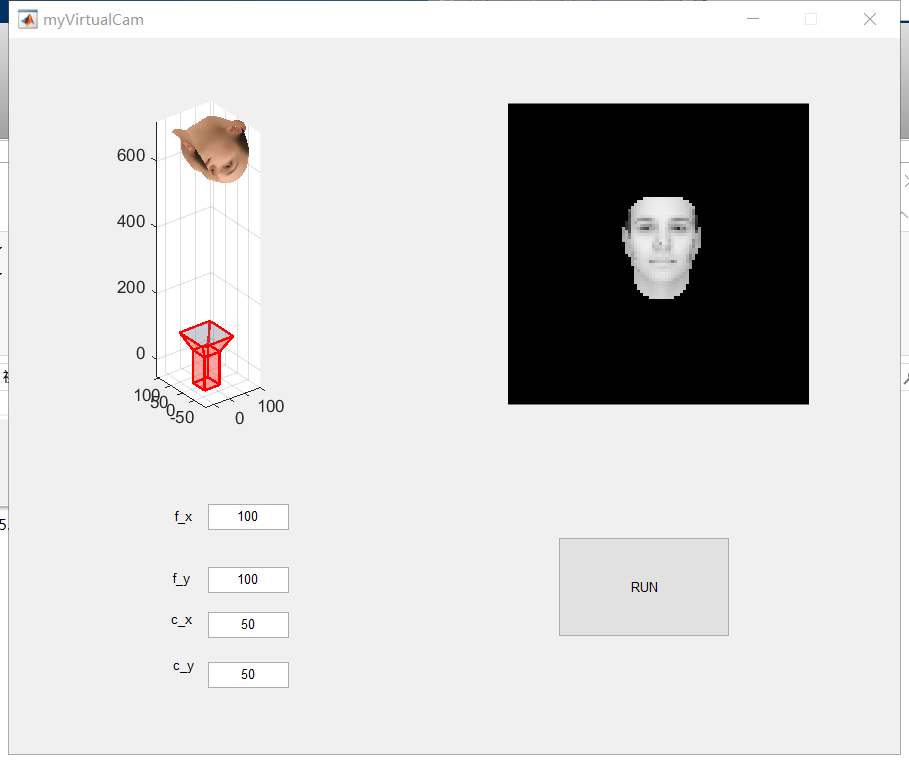
\includegraphics[width=1\textwidth]{fig/1155.png}
	\caption{cx=cy=50\label{fig:1155-}}
\end{minipage}
\hfill
\begin{minipage}[htbp]{0.48\linewidth}
    \centering
	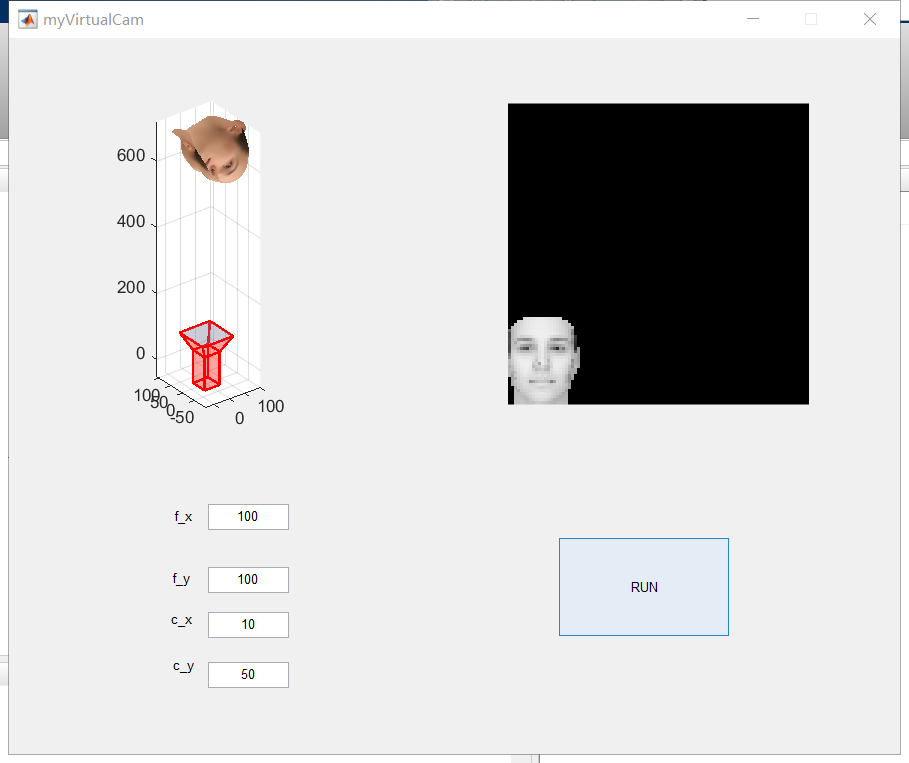
\includegraphics[width=1\textwidth]{fig/1115.png}
	\caption{cx=10,cy=50\label{fig:1115}}
\end{minipage}
\end{figure}
\begin{figure}
\begin{minipage}[htbp]{0.48\linewidth}
    \centering
	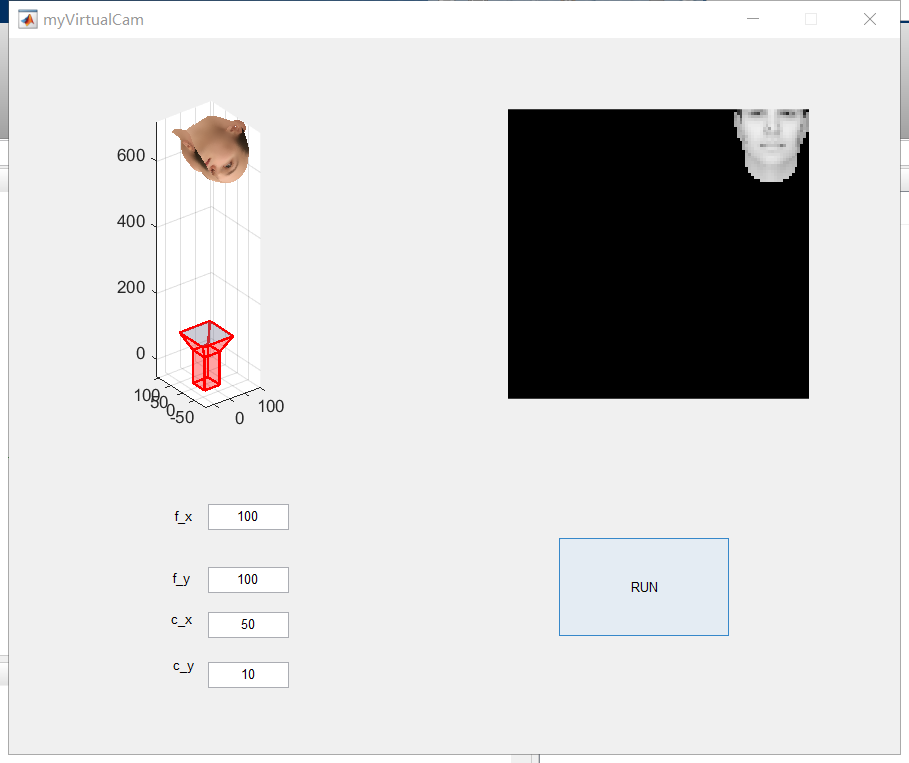
\includegraphics[width=1\textwidth]{fig/1151.png}
	\caption{fx=50,fy=10\label{fig:1151}}
\end{minipage}
\hfill
\begin{minipage}[htbp]{0.48\linewidth}
    \centering
	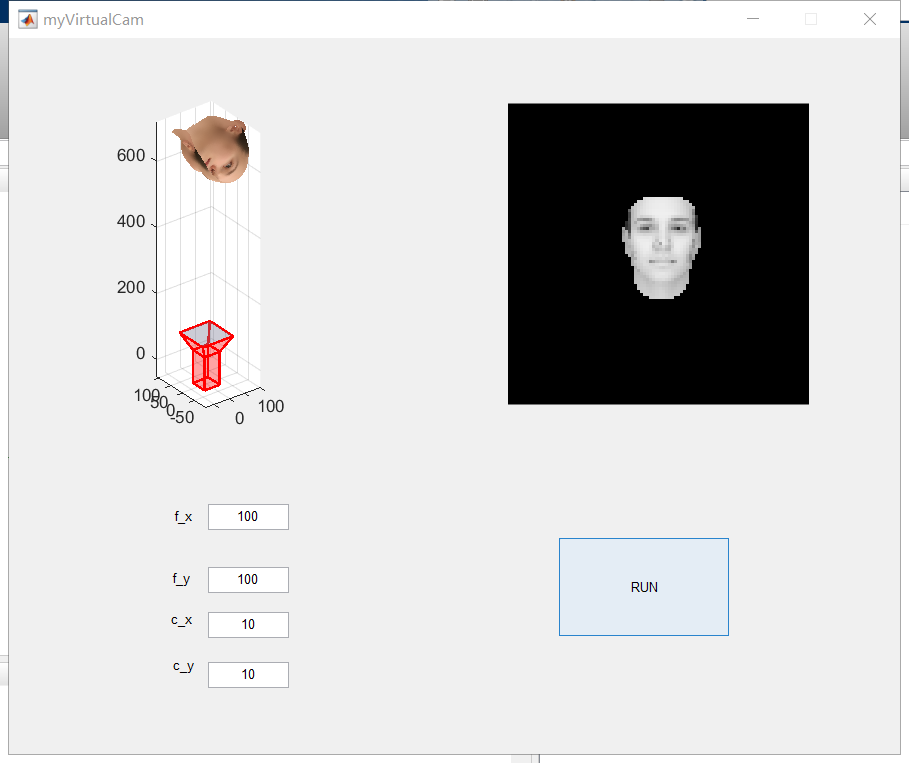
\includegraphics[width=1\textwidth]{fig/1111.png}
	\caption{fx=fy=10\label{fig:1111}}
\end{minipage}
\end{figure}
\end{document}
